\documentclass[a4paper,12pt]{extarticle}
\usepackage[utf8x]{inputenc}
\usepackage[T1,T2A]{fontenc}
\usepackage[russian]{babel}
\usepackage{hyperref}
\usepackage{indentfirst}
\usepackage{listings}
\usepackage{color}
\usepackage{here}
\usepackage{array}
\usepackage{multirow}
\usepackage{graphicx}
\usepackage{algorithm}
\usepackage{algpseudocode}
\usepackage{caption}
\usepackage{pdfpages}
\usepackage{tikz,mathpazo}
\usepackage{graphicx,amssymb,amstext,amsmath,newtxmath}
\usetikzlibrary{shapes.geometric, arrows}
\renewcommand{\lstlistingname}{Программа} % заголовок листингов кода

\bibliographystyle{ugost2008ls}

\usepackage{listings}
\lstset{ %
extendedchars=\true,
keepspaces=true,
language=C,						% choose the language of the code
basicstyle=\footnotesize,		% the size of the fonts that are used for the code
numbers=left,					% where to put the line-numbers
numberstyle=\footnotesize,		% the size of the fonts that are used for the line-numbers
stepnumber=1,					% the step between two line-numbers. If it is 1 each line will be numbered
numbersep=5pt,					% how far the line-numbers are from the code
backgroundcolor=\color{white},	% choose the background color. You must add \usepackage{color}
showspaces=false				% show spaces adding particular underscores
showstringspaces=false,			% underline spaces within strings
showtabs=false,					% show tabs within strings adding particular underscores
frame=single,           		% adds a frame around the code
tabsize=2,						% sets default tabsize to 2 spaces
captionpos=t,					% sets the caption-position to top
breaklines=true,				% sets automatic line breaking
breakatwhitespace=false,		% sets if automatic breaks should only happen at whitespace
escapeinside={\%*}{*)},			% if you want to add a comment within your code
postbreak=\raisebox{0ex}[0ex][0ex]{\ensuremath{\color{red}\hookrightarrow\space}},
texcl=true,
inputpath=listings,                     % директория с листингами
}

\usepackage[left=2cm,right=2cm,
top=2cm,bottom=2cm,bindingoffset=0cm]{geometry}

%% Нумерация картинок по секциям
\usepackage{chngcntr}
\counterwithin{figure}{section}
\counterwithin{table}{section}

%%Точки нумерации заголовков
\usepackage{titlesec}
\titlelabel{\thetitle.\quad}
\usepackage[dotinlabels]{titletoc}

%% Оформления подписи рисунка
\addto\captionsrussian{\renewcommand{\figurename}{Рисунок}}
\captionsetup[figure]{labelsep = period}

%% Подпись таблицы
\DeclareCaptionFormat{hfillstart}{\hfill#1#2#3\par}
\captionsetup[table]{format=hfillstart,labelsep=newline,justification=centering,skip=-10pt,textfont=bf}

%% Путь к каталогу с рисунками
\graphicspath{{fig/}}

%% Внесение titlepage в учёт счётчика страниц
\makeatletter
\renewenvironment{titlepage} {
 \thispagestyle{empty}
}
\makeatother


\begin{document}	% начало документа

% Титульная страница
\begin{titlepage}	% начало титульной страницы

	\begin{center}		% выравнивание по центру

		\large Санкт-Петербургский политехнический университет Петра Великого\\
		\large Физико-механический институт \\
		\large Высшая школа прикладной математики и вычислительной физики\\[3cm]
		% название института, затем отступ 6см
		\large Направление подготовки\\
		\large "01.03.02. Прикладная математика и информатика"\\[3cm]
		\huge Дисциплина "Численные методы"\\[0.5cm] % название работы, затем отступ 0,5см
		\large Отчет по лабораторной работе №3\\[0.1cm]
		\large "Решение СЛАУ итерационными методами. Метод простых итераций"\\[5cm]

	\end{center}


	\begin{flushright} % выравнивание по правому краю
		\begin{minipage}{0.25\textwidth} % врезка в половину ширины текста
			\begin{flushleft} % выровнять её содержимое по левому краю

				\large\textbf{Работу выполнил:}\\
				\large Иванова А.С.\\
				\large {Группа:} 5030102/00002\\
				
				\large \textbf{Преподаватель:}\\
				\large Курц В.В.

			\end{flushleft}
		\end{minipage}
	\end{flushright}
	
	\vfill % заполнить всё доступное ниже пространство

	\begin{center}
	\large Санкт-Петербург\\
	\large \the\year % вывести дату
	\end{center} % закончить выравнивание по центру

\end{titlepage} % конец титульной страницы

\vfill % заполнить всё доступное ниже пространство


% Содержание
\renewcommand\contentsname{\centerline{Содержание}}
\tableofcontents
\newpage



\section{Формулировка задачи}

Решить СЛАУ, используя метод простых итераций. При решении данной задачи будет использоваться одна из модификаций метода простых итераций, а именно метод Якоби. Исследовать точность решения, когда определитель матрицы близок к нулю,ввести один параметр, который уменьшает определитель.
обусловленности. Сравнить решение одинаковых СЛАУ прямыми и итерационными методами при одинаковом объёме вычислений. 

Уравнение в матричном виде 

\begin{math}
	Ax=b
\end{math},
где A - матрица системы, b - столбец свободных членов, x - вектор-столбец неизвестных (который нужно найти)

\section{Алгоритм метода и условия его применимости}

\subsection {Условия применимости}

Матрица системы должна быть невырожденной (определитель матрицы не должен равняться 0)

Матрица системы должна обладать свойством диагонального преобладания по строкам 

\subsection {Алгоритм метода}

Дана СЛАУ 
\begin{math}
	Ax=b
\end{math}

Необходимо привести ее к виду, удобному для итераций
\begin{math}
	x=Cx+g
\end{math}

\begin{math}
	x^{(k+1)}=Cx^{(k)}+g
\end{math}

Метод является стационарным, следовательно матрица C и столбец g постоянны.

\begin{math}
	Ax=b <=> -\alpha(Ax-b),\alpha\ne 0 <=> Bx=Bx-\alpha(Ax-b), \det{B}\ne 0
\end{math}

\begin{math}
	x^{(k+1)}=x^{(k)}-\alpha B^{-1}(Ax-b)<=>x=(E-\alpha B^{-1}A)x+\alpha B^{-1} b
\end{math}

\begin{math}
   B\frac{x^{(k+1)}-x^{(k)}}{\alpha}+Ax^{(k)}=b
\end{math}

\begin{math}
	\alpha=1,B=D=diag(A)
\end{math}

\begin{math}
		x^{(k+1)}=x^{(k)}-D^{-1}(Ax^{(k)}-b)=(E-D^{-1}A)x^{(k)}+D^{-1}b
\end{math}


Таким образом: 

\begin{math}
	E-D^{-1}A=C
\end{math}

\begin{math}
	D^{-1}b=g
\end{math}

Тогда eсли i=j, то 
\begin{math}
	c_{ij}=0
\end{math}
, если нет, то
\begin{math}
	c_{ij}=-a_{ij}/a_{ii}
\end{math}

Критерий остановки итерационного процесса 

\begin{math}
	||x^{(k)}-x^{(k-1)}||<\frac{1-||C||}{||C||}\epsilon
\end{math}


\section{Предварительный анализ задачи}

Матрицы генерируются в системе MATLAB таким образом, что точно выполняется условие диагонального преобладания по строкам (элементы на главной диагонали матрицы системы на несколько порядков больше остальных элементов).

\section{Проверка условий применимости метода}

Матрицы генерируются в системе MATLAB таким образом, что точно выполняется условие диагонального преобладания по строкам (элементы на главной диагонали матрицы системы на несколько порядков больше остальных элементов).

\section{Тестовый пример с детальными расчетами для задачи малой размерности}

Решим систему уравнений с точностью до 10e-4

\begin{equation*}
	\begin{cases}
		10x_{1}+x_{2}-x_{3}&=11\\
		x_{1}+10x_{2}-x_{3}&=10\\
		-x_{1}+x_{2}+10x_{3}&=10
	\end{cases}
\end{equation*}

Найдем определитель матрицы системы, чтобы убедиться, что она невырожденная 

\begin{equation*}
	\det A =
	\begin{vmatrix}
		10 & 1 & -1\\
		1 & 10 & -1\\
		-1 & 1 & 10
	\end{vmatrix}
	= 990
\end{equation*}

Наглядно видно, что данная матрица обладает свойством диагонального преобладания по строкам

Точное решение:

\begin{equation*}
	x =
	\begin{pmatrix}
		\frac{1091}{990}\\
		\frac{109}{110}\\
		\frac{91}{90}
	\end{pmatrix}
\end{equation*}

Данная система имеет единственное решение.

Приводим СЛАУ к удобному виду для итерации:

\begin{equation*}
	\begin{cases}
		x_{1}&=-0,1x_{2}+0,1x_{3}+1,1\\
		x_{2}&=-0,1x_{1}+0,1x_{3}+1\\
		x_{3}&=0,1x_{1}-0,1x_{2}+1
	\end{cases}
\end{equation*}

Выберем начальное приближение

\begin{equation*}
	x^{(0)} =
	\begin{pmatrix}
		1,1\\
		1\\
		1
	\end{pmatrix}
\end{equation*}

\begin{equation*}
	\begin{cases}
		x_{1}^{(1)}&=-0,1*1+0,1*1+1,1\\
		x_{2}^{(1)}&=-0,1*1,1+0,1+1\\
		x_{3}^{(1)}&=0,1*1,1-0,1*1+1
	\end{cases}
\end{equation*}

Таким образом первое приближение:

\begin{equation*}
	x^{(1)} =
	\begin{pmatrix}
		1,1\\
		0,99\\
		1,01
	\end{pmatrix}
\end{equation*}

Далее производятся аналогичные вычисления для следующих итераций

\begin{equation*}
	x^{(2)} =
	\begin{pmatrix}
		1,102\\
		0,991\\
		1,011
	\end{pmatrix}
\end{equation*}

\begin{equation*}
	x^{(3)} =
	\begin{pmatrix}
		1,102\\
		0,9909\\
		1,0111
	\end{pmatrix}
\end{equation*}

\begin{equation*}
	x^{(4)} =
	\begin{pmatrix}
		1,10202\\
		0,99091\\
		1,01111
	\end{pmatrix}
\end{equation*}

Проверим, достиглась ли нужная точность

\begin{math}
	||x^{(4)}-x^{(3)}||_{\infty}=2*10^{-5}
\end{math}

\begin{math}
	||C||_{\infty}=0.2
\end{math}

\begin{math}
	\frac{1-||C||}{||C||}*0,0001=0.0004
\end{math}


\begin{math}
	2*10^{-5}<0,0004
\end{math}

Нужная точность достигнута
\section{Перечень контрольных тестов для иллюстрации метода}

\subsection{Исследование точности решения при определителе, близком к нулю}

Точное решение СЛАУ везде одинаковое (столбец единиц). Размерность матрицы фиксирована (15 на 15)

Выявляется две зависимости: относительная погрешность от определителя при фиксированном количестве итераций (в данном случае 3) и количества итераций, необходимого для достижения точности 10е-15 от определителя. 

Ожидается, что при меньшем определителе погрешность будет больше и что чем определитель матрицы ближе к нулю, тем большее количество итераций требуется для нахождения корней с заданной точностью.

Генерируется матрица следующим образом: элементы на главной диагонали как 100*rand(), остальные элементы как rand()*0.0000001. Задается массив для изменения матрицы [1 0.5 0.1 0.05 0.01 0.005 0.001 0.0005 0.0001 0.00005 0.00001]. Все диагональные элементы умножаются на элементы данного массива, таким образом получается 11 матриц, в каждой последующей определитель на несколько порядков меньше, чем у предыдущей. Вычисляются определители этих матриц. 

\subsection{Сравнение решения одинаковых СЛАУ прямыми и итерационными методами}

Генерируется 99 матриц с разными размерами с диагональным преобладанием. Элементы на главной диагонали генерируются как 10000*rand(), остальные элементы как rand() * 0.00001. Размер матрицы меняется в цикле от 10 до 500 с шагом 5. Сравниваются решения прямым методом вращений и методом простых итераций (модификацией методом Якоби). Ожидается, что для решения систем с большой размерностью итерационный метод якоби покажет лучшие результаты, чем прямой метод вращений. Для метода простых итераций выбрана точность 10е-15, примерно с такой точностью вычисляются корни методом вращений при хорошо обусловленной матрице. 

\section{Модульная структура программы}

Функция long double** ArrayRead(FILE* file, int line, int column)

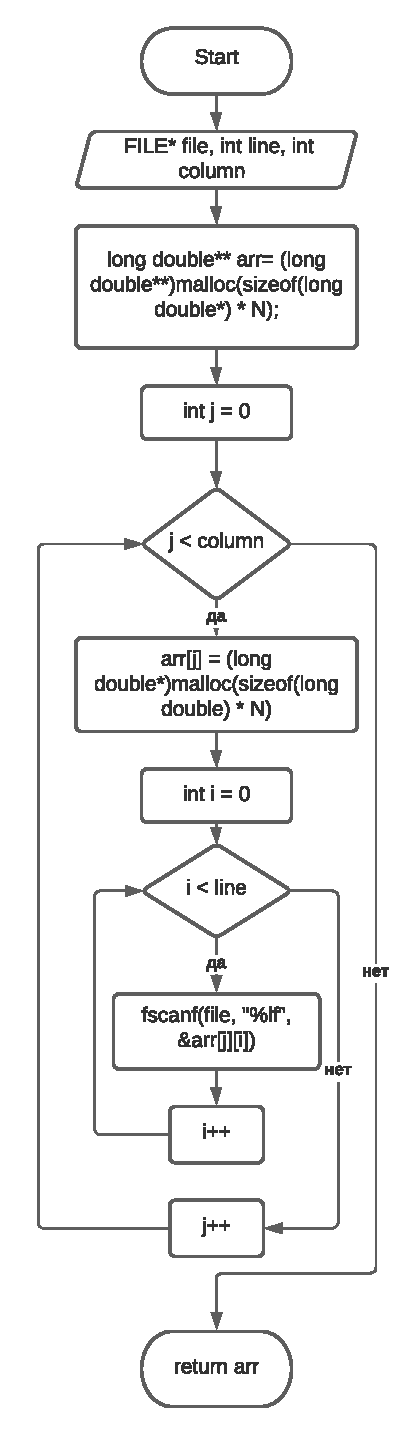
\includegraphics[scale=0.5]{block1.pdf}

Функция long double* ColumnRead(FILE* file, int size)

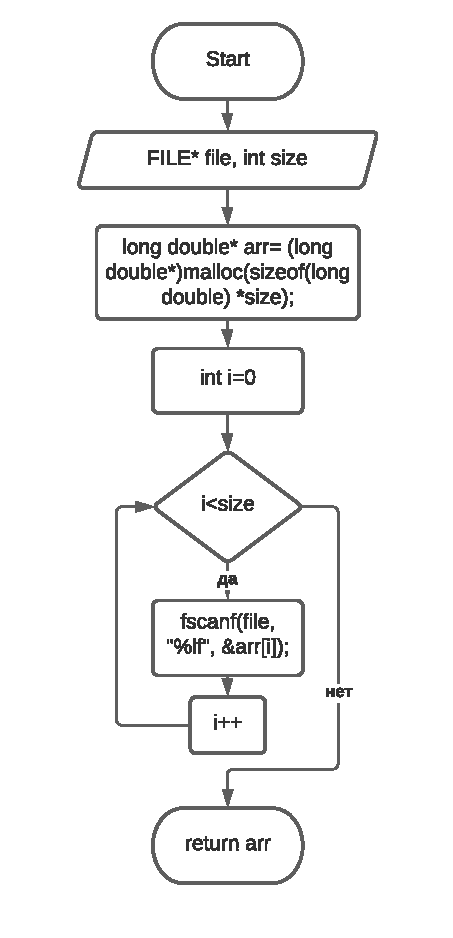
\includegraphics[scale=0.5]{block2.pdf}

Функция long double** CreatePrecondMatrix(long double** A, int size)

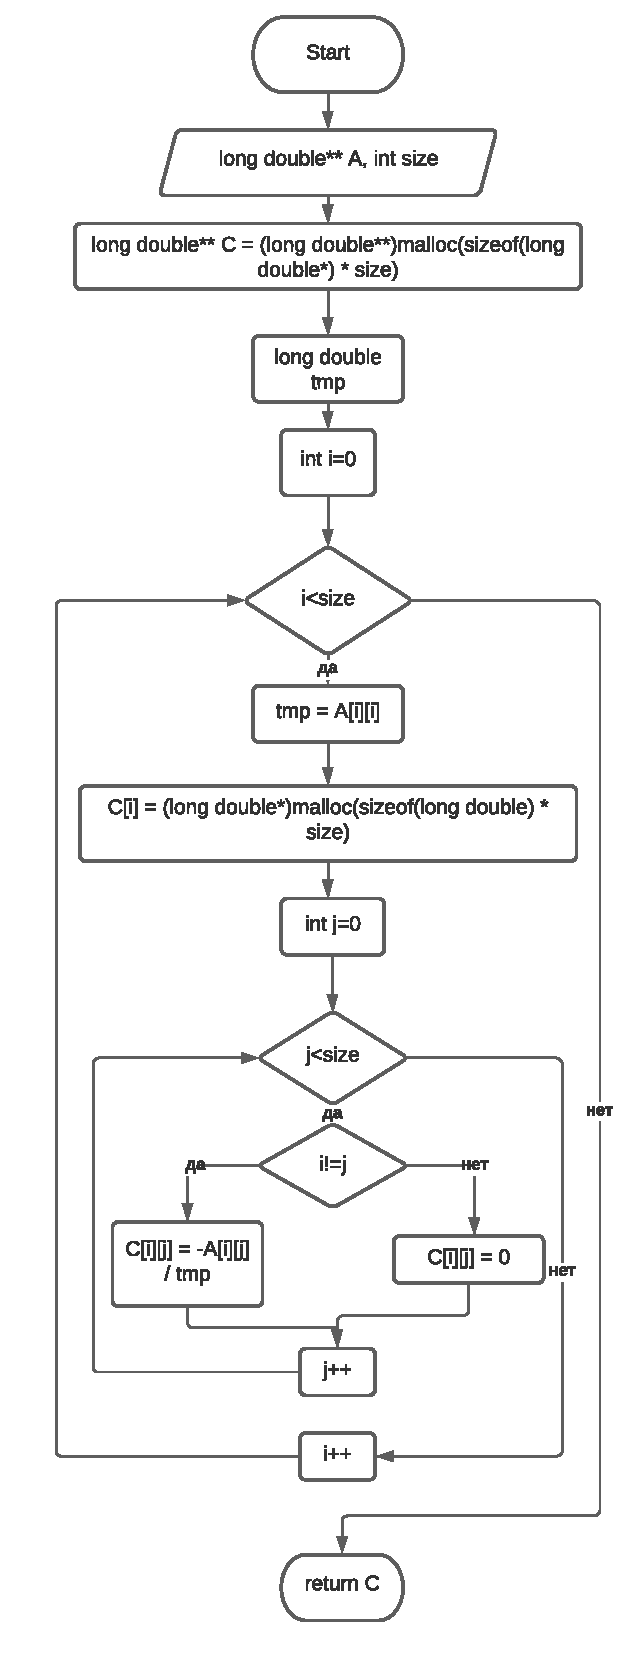
\includegraphics[scale=0.5]{block3.pdf}

Функция long double NormMatrix(long double** matrix,int size)

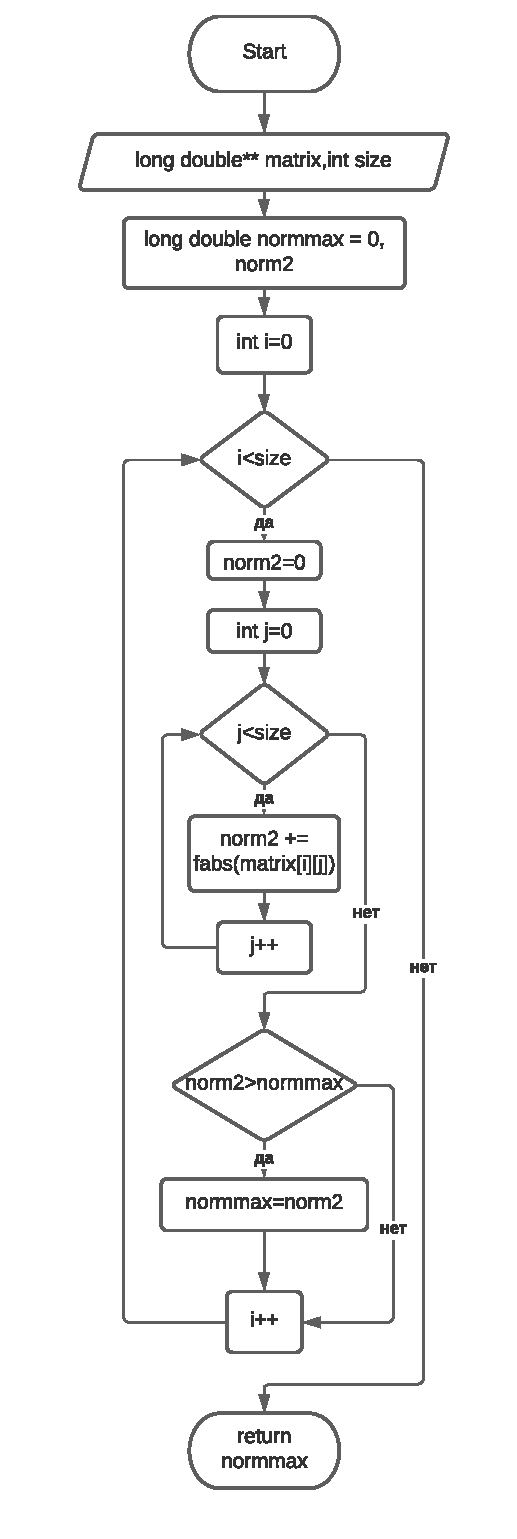
\includegraphics[scale=0.5]{block4.pdf}

Функция long double* ZeroApproximate(long double** A, long double* b, int size)

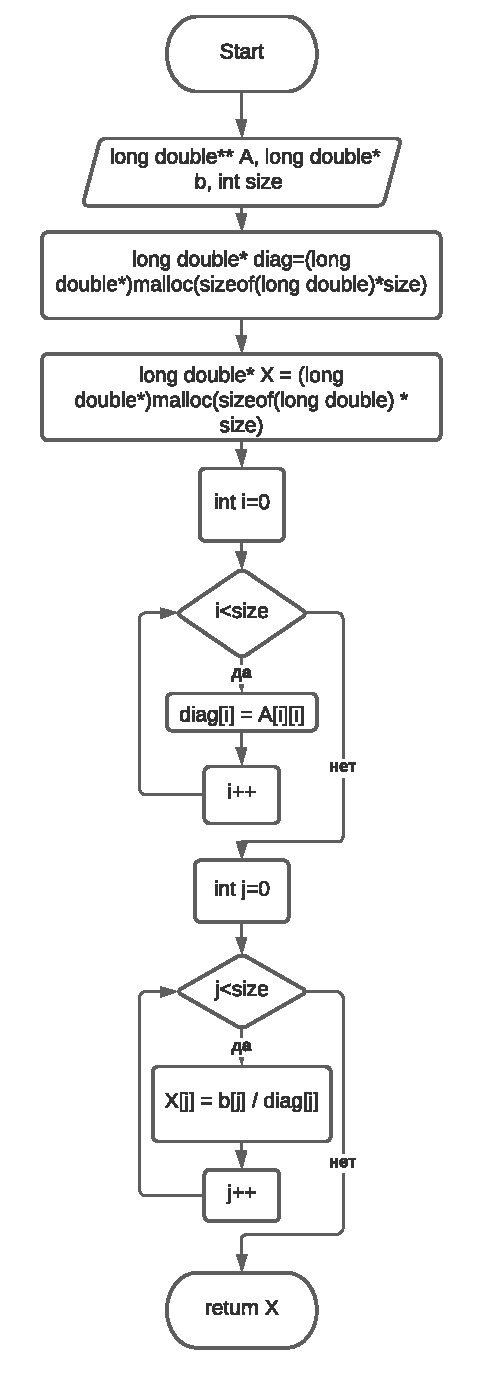
\includegraphics[scale=0.5]{block5.pdf}

Функция void Jacobi(long double** A, long double* b, int size)

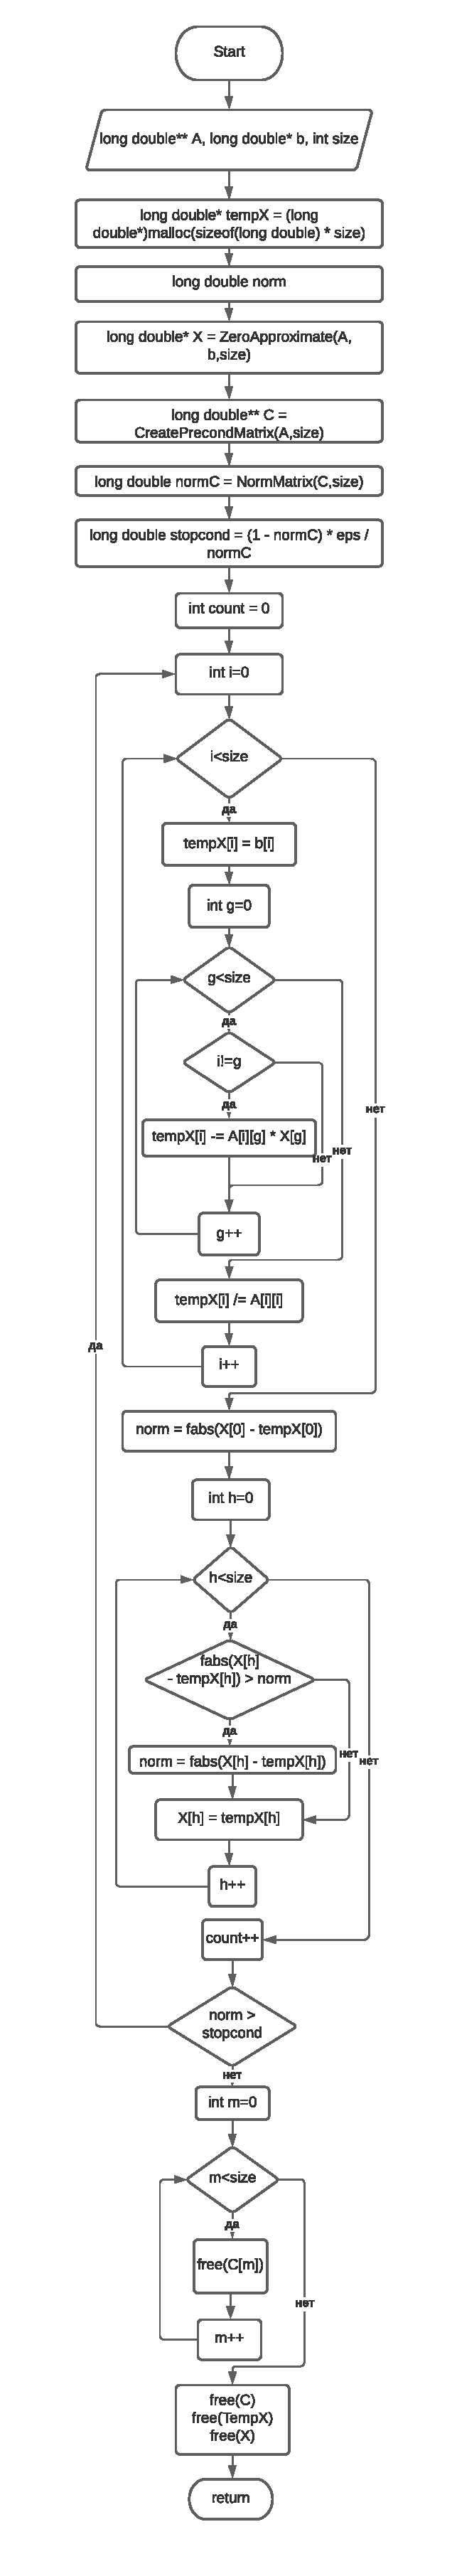
\includegraphics[scale=0.4]{block6.pdf}

\section{Численный анализ решения задачи}

\subsection{Исследование точности решения при определителе, близком к нулю}

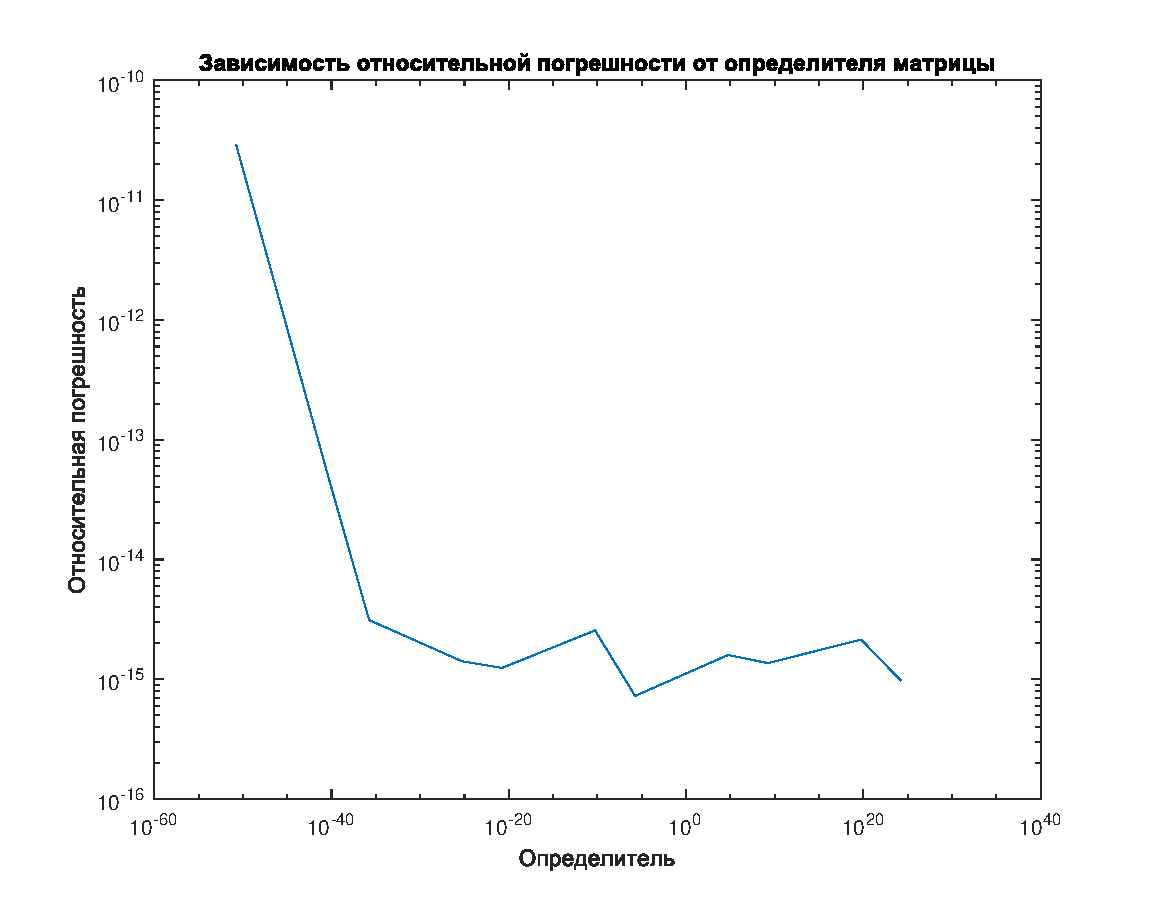
\includegraphics[scale=0.5]{5.pdf}

Данный график отображает зависимость относительной погрешности вычисления за три итерации от определителя матрицы. Из графика видно, что чем определитель ближе к нулю, тем больше погрешность.

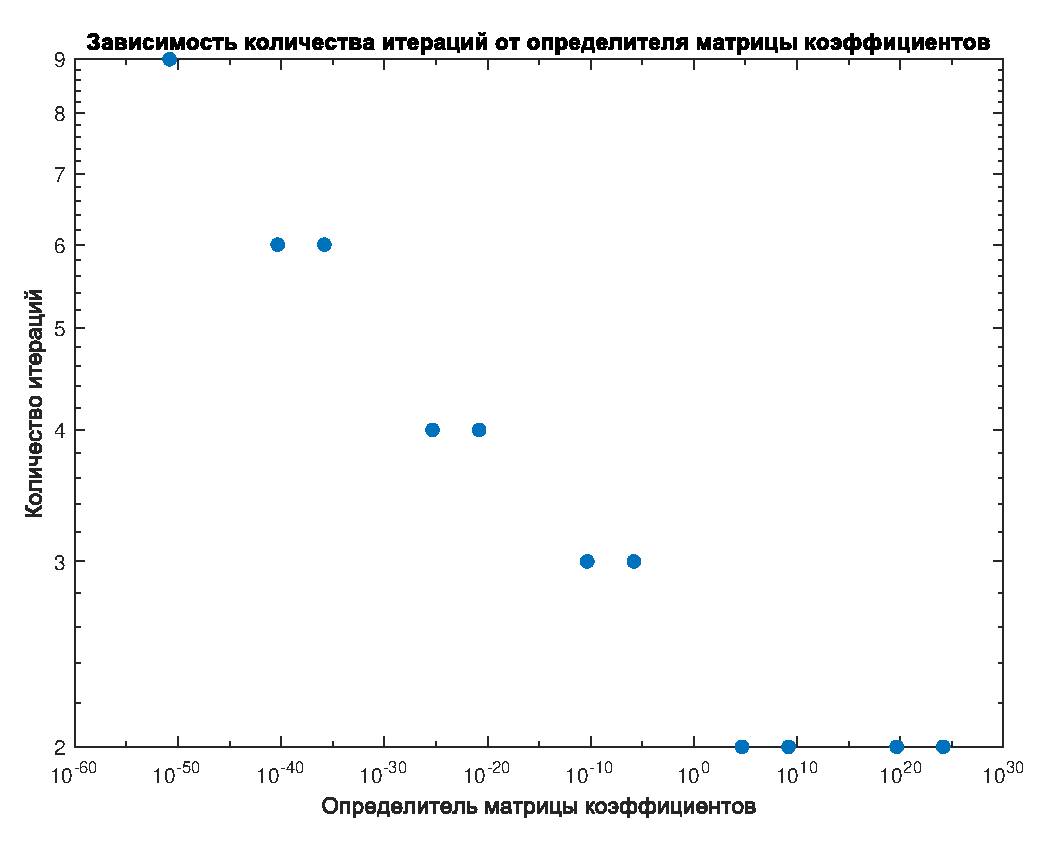
\includegraphics[scale=0.5]{2.pdf}

Данный график отображает зависимость количества итераций, необходимого для достижения заданной точности вычислений от определителя матрицы коэффициентов. Зависимость напоминает линейную в логарифмическом масшатбе, можно сделать вывод, что при приближении определителя к нулю, необходимое количество итераций, необходимое для вычисления корней увеличивается.

\subsection{Сравнение решения одинаковых СЛАУ прямыми и итерационными методами}

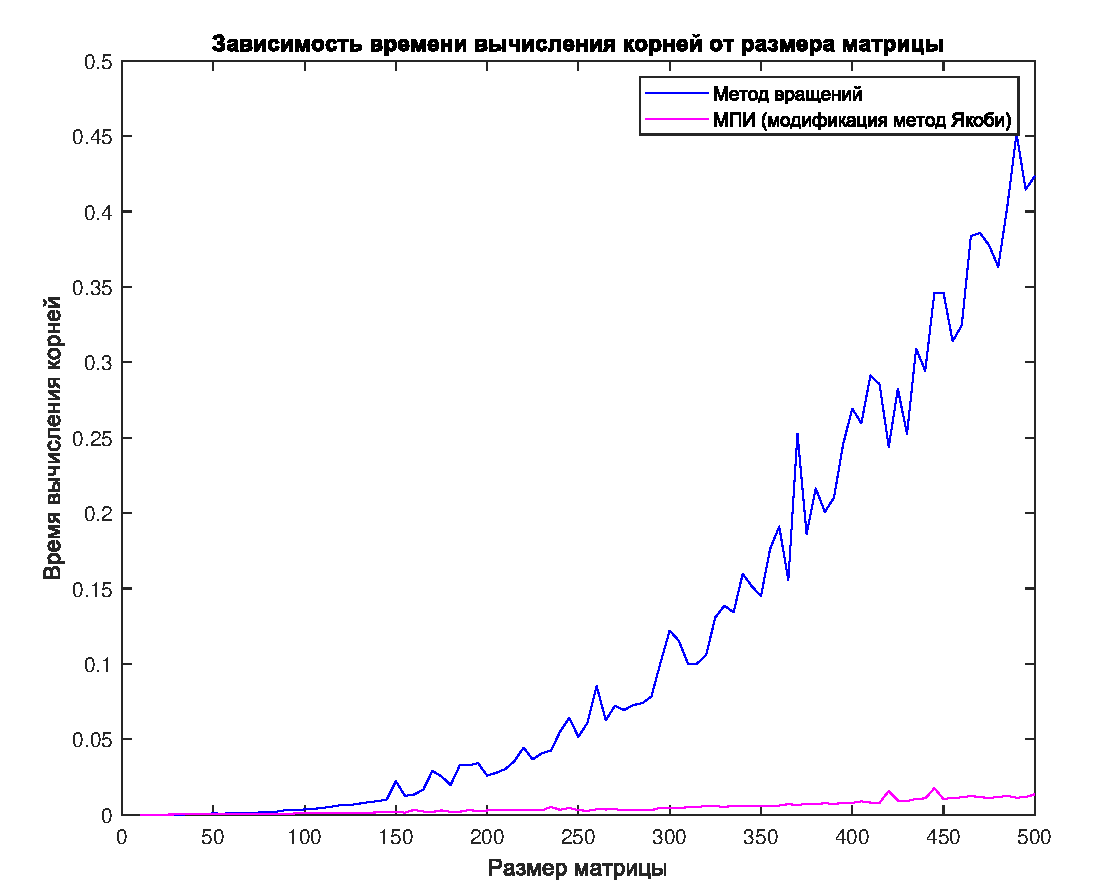
\includegraphics[scale=0.5]{3.pdf}

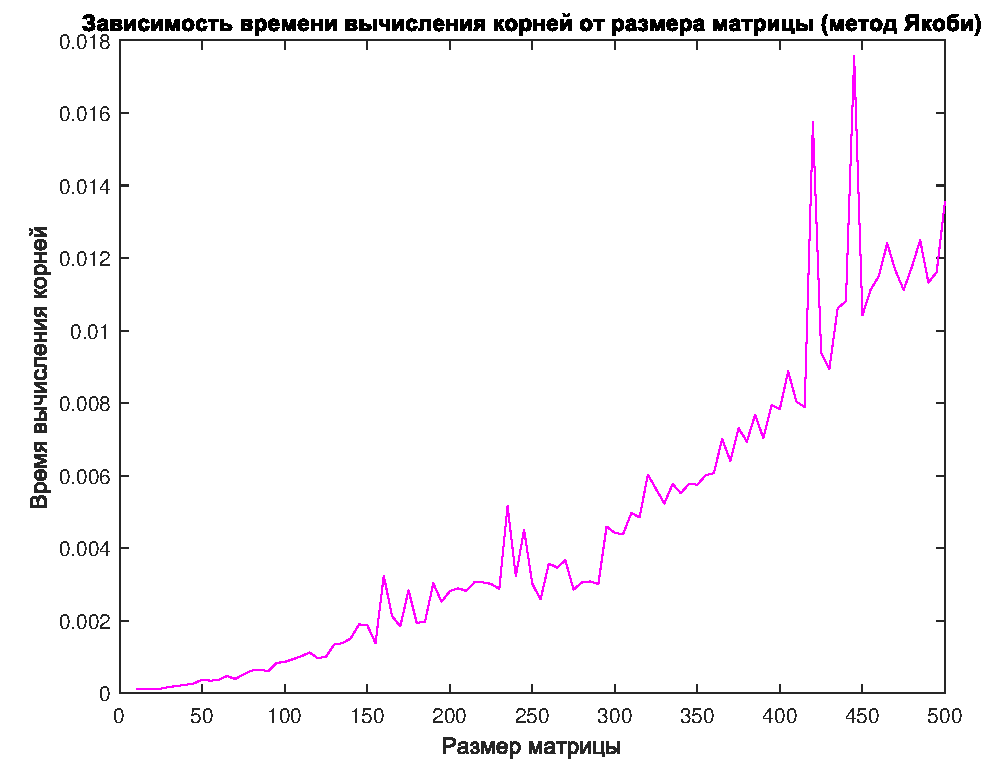
\includegraphics[scale=0.5]{4.pdf}

Из данных графиков видно, что с ростом размерности системы время, необходимое для вычисления корней при решении прямым методом вращений растет гораздо быстрее, чем при решении методом простых итераций. Для метода вращений зависимость близка к кубической, а для метода простых итераций близка к квадратичной. 

\section{Краткие выводы}

Была решена задача нахождения корней СЛАУ одной из модификаций метода простых итераций - методом Якоби.

Была исследована точность решения при определителе матрицы системы, близком к нулю.

Было произведено сравнение итерационного метода Якоби и прямого метода вращений, с помощью чего было подтверждено, что для систем с большой размерностью лучше использовать итерационные методы нахождения корней.

\end{document}
